% =============================================================================
%  MANUAL DE USUARIO — EQUIPO DE PRÁCTICAS DE CONTROL DE MOTOR CC
%  Departamento de Ingeniería de Sistemas y Automática (ISA)
%  Universidad de Sevilla
%  Contacto: ialvarado@us.es
% =============================================================================
\documentclass[11pt,a4paper]{article}

% ── Codificación y lengua ────────────────────────────────────────────────────
\usepackage[utf8]{inputenc}
\usepackage[T1]{fontenc}
\usepackage[english]{babel}
\selectlanguage{english}

% ── Tipografía ───────────────────────────────────────────────────────────────
\usepackage{lmodern}
\usepackage{microtype}

% ── Márgenes ─────────────────────────────────────────────────────────────────
\usepackage[top=2.5cm,bottom=2.5cm,left=2.5cm,right=2.5cm]{geometry}

% ── Gráficos y color ─────────────────────────────────────────────────────────
\usepackage{graphicx}
\usepackage[table,xcdraw]{xcolor}
\usepackage{tikz}
\usetikzlibrary{shapes.geometric,arrows.meta,positioning,fit,backgrounds,calc}

% ── Tablas ───────────────────────────────────────────────────────────────────
\usepackage{booktabs}
\usepackage{array}
\usepackage{multirow}
\usepackage{longtable}

% ── Código fuente ────────────────────────────────────────────────────────────
\usepackage{listings}
\usepackage{courier}

% ── Cajas y advertencias ─────────────────────────────────────────────────────
\usepackage{tcolorbox}
\tcbuselibrary{skins,breakable}

% ── Iconos / símbolos ────────────────────────────────────────────────────────
\usepackage{pifont}
\usepackage{amssymb}
% Sustitutos de fontawesome5
\newcommand{\faInfoCircle}{$\blacksquare$}
\newcommand{\faExclamationTriangle}{$\triangle$}
\newcommand{\faCheckCircle}{\ding{52}}
\newcommand{\faTimesCircle}{\ding{56}}
\newcommand{\faUpload}{$\uparrow$}
\newcommand{\faPlay}{$\blacktriangleright$}

% ── Hiperenlaces ─────────────────────────────────────────────────────────────
\usepackage[colorlinks=true,linkcolor=isablue,urlcolor=isablue,citecolor=isablue]{hyperref}

% ── Encabezados y pie de página ──────────────────────────────────────────────
\usepackage{fancyhdr}
\usepackage{lastpage}

% ── Listas mejoradas ─────────────────────────────────────────────────────────
\usepackage{enumitem}

% ── Espaciado entre párrafos ─────────────────────────────────────────────────
\setlength{\parskip}{4pt}
\setlength{\parindent}{0pt}

% =============================================================================
%  COLORES ISA
% =============================================================================
\definecolor{isablue}{RGB}{0,70,130}
\definecolor{isared}{RGB}{180,30,30}
\definecolor{isagray}{RGB}{240,242,244}
\definecolor{isagreen}{RGB}{0,120,60}
\definecolor{isaorange}{RGB}{200,90,0}
\definecolor{codebg}{RGB}{248,248,248}

% =============================================================================
%  CAJAS DE AVISO
% =============================================================================
\newtcolorbox{infobox}[1][]{
  colback=isablue!8, colframe=isablue, fonttitle=\bfseries,
  title={\faInfoCircle\quad Nota}, #1
}
\newtcolorbox{warnbox}[1][]{
  colback=isaorange!10, colframe=isaorange, fonttitle=\bfseries,
  title={\faExclamationTriangle\quad Atención}, #1
}
\newtcolorbox{successbox}[1][]{
  colback=isagreen!8, colframe=isagreen, fonttitle=\bfseries,
  title={\faCheckCircle\quad Correcto}, #1
}
\newtcolorbox{errorbox}[1][]{
  colback=isared!8, colframe=isared, fonttitle=\bfseries,
  title={\faTimesCircle\quad Problema frecuente}, #1
}

% =============================================================================
%  ESTILO DE CÓDIGO
% =============================================================================
\lstset{
  basicstyle=\ttfamily\small,
  backgroundcolor=\color{codebg},
  frame=single,
  rulecolor=\color{gray!40},
  breaklines=true,
  columns=fullflexible,
  keepspaces=true,
  showstringspaces=false,
  numbers=none,
}
\lstdefinestyle{matlab}{language=Matlab, keywordstyle=\color{isablue}\bfseries,
  commentstyle=\color{gray}\itshape, stringstyle=\color{isared}}
\lstdefinestyle{bash}{language=bash, keywordstyle=\color{isagreen}\bfseries,
  commentstyle=\color{gray}\itshape}

% =============================================================================
%  ENCABEZADO / PIE
% =============================================================================
\pagestyle{fancy}
\fancyhf{}
\fancyhead[L]{\textcolor{isablue}{\small\textbf{Manual de usuario — Equipo motor CC}}}
\fancyhead[R]{\textcolor{isablue}{\small ISA · Universidad de Sevilla}}
\fancyfoot[C]{\textcolor{gray}{\small Página \thepage\ de \pageref{LastPage}}}
\renewcommand{\headrulewidth}{0.4pt}
\renewcommand{\footrulewidth}{0pt}
\renewcommand{\headrule}{\color{isablue}\hrule width\headwidth height\headrulewidth}

% =============================================================================
%  TÍTULO
% =============================================================================
\title{%
  \vspace{-1cm}
  {\color{isablue}\rule{\linewidth}{2pt}}\\[0.5em]
  {\Huge\bfseries\color{isablue} Manual de Usuario}\\[0.3em]
  {\Large Equipo de Prácticas de Control de Motor CC}\\[0.3em]
  {\color{isablue}\rule{\linewidth}{0.5pt}}\\[0.3em]
  {\normalsize Departamento de Ingeniería de Sistemas y Automática (ISA)\\
   Universidad de Sevilla \quad·\quad \href{mailto:ialvarado@us.es}{ialvarado@us.es}}
}
\date{\today}
\author{}

% =============================================================================
\begin{document}
% =============================================================================

\maketitle
\thispagestyle{fancy}

% ── Resumen rápido ─────────────────────────────────────────────────────────
\begin{tcolorbox}[colback=isablue!5,colframe=isablue,fontupper=\small]
\textbf{En qué consiste este equipo:} un motor DC Maxon con encoder magnético de 14 bits,
controlado en lazo cerrado desde MATLAB/Simulink a través de un Arduino.
El lazo de control \emph{corre íntegramente en el PC}: Arduino solo lee el encoder y aplica
el PWM que MATLAB le ordena cada \textbf{10 ms} (100 Hz). La comunicación es por
USB/serie a 115 200 baudios.

\medskip
\textbf{Lo que necesita el profesor:} conectar el USB, identificar el puerto serie
en MATLAB, y lanzar el experimento. El resto es automático.
\end{tcolorbox}

\tableofcontents
\newpage

% =============================================================================
\section{Descripción del equipo}
% =============================================================================

\subsection{Componentes principales}

\begin{center}
\begin{tabular}{llp{7.5cm}}
\toprule
\textbf{Componente} & \textbf{Modelo} & \textbf{Función} \\
\midrule
Motor & Maxon A-max 22 & Motor DC de precisión con reductora planetaria GP 22 B \\
Encoder & ams AS5047P & Encoder magnético 14 bits (16\,384 pasos/vuelta), montado en el lado de carga \\
Driver & TB6612FNG & Driver de motor dual integrado en la placa shield \\
Microcontrolador & Arduino UNO & Lee el encoder, aplica PWM y se comunica con MATLAB por USB \\
Placa shield & ISA custom & Apilable sobre el Arduino; integra driver + conector encoder \\
\bottomrule
\end{tabular}
\end{center}

\subsection{Esquema de conexiones}

\begin{center}
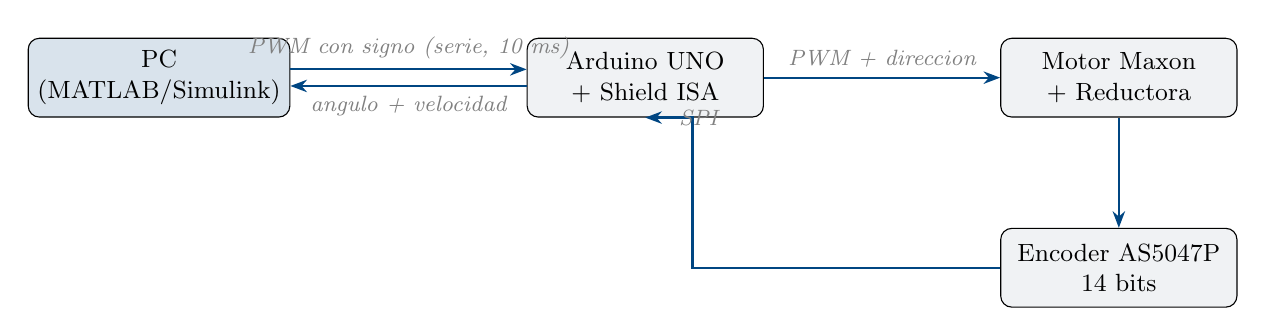
\begin{tikzpicture}[
  block/.style={draw,rounded corners,fill=isagray,minimum width=3cm,minimum height=1cm,
                align=center,font=\small},
  arrow/.style={-{Stealth[length=6pt]},thick,isablue},
  label/.style={font=\footnotesize\itshape,text=gray}
]
  \node[block,fill=isablue!15] (pc)     {PC\\(MATLAB/Simulink)};
  \node[block,right=3cm of pc]  (ard)   {Arduino UNO\\+ Shield ISA};
  \node[block,right=3cm of ard] (mot)   {Motor Maxon\\+ Reductora};
  \node[block,below=1.4cm of mot](enc)  {Encoder AS5047P\\14 bits};

  \draw[arrow] ([yshift=3pt]pc.east)  -- node[above,label]{PWM con signo (serie, 10 ms)} ([yshift=3pt]ard.west);
  \draw[arrow] ([yshift=-3pt]ard.west)-- node[below,label]{angulo + velocidad} ([yshift=-3pt]pc.east);
  \draw[arrow] (ard.east)  -- node[above,label]{PWM + direccion} (mot.west);
  \draw[arrow] (enc.west)  -| ([xshift=0.6cm]ard.south) -- node[right,label,pos=0.5]{SPI} (ard.south);
  \draw[arrow] (mot.south) -- (enc.north);
\end{tikzpicture}
\end{center}

\begin{infobox}
El lazo de control completo reside en MATLAB. Arduino actúa únicamente como
\textbf{interfaz hardware}: lee el encoder por SPI, calcula la velocidad como diferencia
de posición dividida por $T_s = 0.01$ s, y aplica la señal de control al driver.
\end{infobox}

\subsection{Parámetros del sistema}

\begin{center}
\begin{tabular}{lll}
\toprule
\textbf{Parámetro} & \textbf{Valor} & \textbf{Notas} \\
\midrule
Periodo de muestreo $T_s$ & 10 ms (100 Hz) & Fijado en el firmware de Arduino \\
Velocidad de comunicación & 115\,200 baudios & USB/serie \\
Rango señal de control & $u \in [-255,\,255]$ & Equivale a $\pm$12 V \\
Resolución encoder & $\approx 0.022°$/paso & 16\,384 pasos/vuelta \\
Modelo aproximado & $G(s)=K/(\tau s+1)$ & $K\approx3$, $\tau\approx0.07$ s a 12 V \\
\bottomrule
\end{tabular}
\end{center}

% =============================================================================
\section{Puesta en marcha inicial (una sola vez)}
% =============================================================================

Esta sección solo es necesaria la \textbf{primera vez} que se configura el equipo,
o si se cambia el Arduino. No hace falta repetirla en cada sesión de prácticas.

\subsection{Instalar las librerías de Arduino}

\begin{enumerate}[leftmargin=*]
  \item Abrir \textbf{Arduino IDE 2.x}.
  \item Ir a \texttt{Herramientas → Gestor de librerías}.
  \item Buscar e instalar \texttt{AS5047P} (autor: Marginally Clever Robots).
  \item Buscar e instalar \texttt{MsTimer2} (autor: Javier Valencia).
\end{enumerate}

\begin{infobox}
Estas librerías solo se instalan una vez en el PC del laboratorio.
Si se cambia de ordenador, hay que repetir este paso.
\end{infobox}

\subsection{Cargar el firmware en el Arduino}

\begin{enumerate}[leftmargin=*]
  \item Conectar el Arduino al PC por USB.
  \item Abrir el archivo \texttt{firmware/arduino/main/main.ino} del repositorio.
  \item Seleccionar la placa correcta: \texttt{Herramientas → Placa → Arduino UNO}.
  \item Seleccionar el puerto: \texttt{Herramientas → Puerto → COMx} (Windows) o
        \texttt{/dev/tty.usbmodem…} (Mac/Linux).
  \item Pulsar el botón \faUpload\ \textbf{Subir} (o \texttt{Ctrl+U}).
  \item Esperar a que aparezca el mensaje \emph{``Subida exitosa''}.
\end{enumerate}

\begin{successbox}
Para verificar que el firmware funciona: abrir el \textbf{Monitor Serie} del IDE
(\texttt{Ctrl+Shift+M}), configurarlo a \texttt{115200 baudios}. Deben aparecer caracteres
binarios (datos en crudo) a 100 Hz. Si no aparece nada, revisar el cableado del encoder.
\end{successbox}

\begin{warnbox}
El firmware ya está cargado en el equipo del laboratorio. Solo hay que volver
a cargarlo si se reemplaza el Arduino o se actualiza el firmware.
\end{warnbox}

\subsection{Comprobar el cableado de la placa shield}

La placa shield se apila directamente sobre el Arduino (conexión sin cables).
Verificar que:

\begin{itemize}[leftmargin=*]
  \item La shield está bien asentada sobre el Arduino (todos los pines encajados).
  \item El cable del motor está conectado a los bornes del driver.
  \item El cable del encoder (conector JST de 7 pines) está conectado a la shield.
  \item La alimentación de 12 V está conectada al borne de la shield.
\end{itemize}

% =============================================================================
\section{Uso en cada sesión de prácticas}
% =============================================================================

Este es el procedimiento habitual al inicio de cada sesión. Con el equipo
ya configurado, tarda menos de dos minutos.

\subsection{Paso 1 — Conectar el hardware}

\begin{enumerate}[leftmargin=*]
  \item Conectar el cable USB del Arduino al PC.
  \item Conectar la fuente de alimentación de 12 V al equipo (borne de la shield).
  \item El LED del Arduino debe encenderse. \faCheckCircle
\end{enumerate}

\begin{warnbox}
Conectar siempre primero el USB y \emph{después} la alimentación de 12 V.
Al desconectar, en orden inverso: primero la alimentación, luego el USB.
\end{warnbox}

\subsection{Paso 2 — Identificar el puerto serie en MATLAB}

\begin{enumerate}[leftmargin=*]
  \item Abrir MATLAB.
  \item Ejecutar en la ventana de comandos:
\end{enumerate}

\begin{lstlisting}[style=matlab]
serialportlist("available")
\end{lstlisting}

MATLAB devolverá algo parecido a:

\begin{lstlisting}
ans =
  "/dev/tty.usbmodem1101"    % Mac
  "COM5"                     % Windows
\end{lstlisting}

\begin{enumerate}[leftmargin=*,start=3]
  \item Anotar el nombre del puerto del Arduino (normalmente el único nuevo que aparece
        al conectar el USB).
\end{enumerate}

\begin{infobox}
En el archivo \texttt{software/matlab/config.m} hay un parámetro \texttt{PORT} que
hay que actualizar con este valor si es diferente al configurado.
El modelo Simulink \texttt{MotorCC\_V2.slx} detecta el puerto automáticamente en Mac/Linux;
en Windows puede ser necesario configurarlo manualmente en ese archivo.
\end{infobox}

\subsection{Paso 3 — Lanzar el experimento desde MATLAB}

\subsubsection*{Opción A: Script MATLAB (identificación / control manual)}

\begin{enumerate}[leftmargin=*]
  \item Abrir \texttt{software/matlab/config.m} y verificar/ajustar \texttt{PORT}.
  \item Ejecutar el script correspondiente:
\end{enumerate}

\begin{lstlisting}[style=matlab]
run('config.m')           % Cargar parametros globales
run('identificacion.m')   % Experimento de identificacion por escalon
% o bien:
run('main_control.m')     % Lazo de control en tiempo real
\end{lstlisting}

\subsubsection*{Opción B: Modelo Simulink}

\begin{enumerate}[leftmargin=*]
  \item Abrir \texttt{software/matlab/MotorCC\_V2.slx}.
  \item Pulsar el botón \textbf{Run} (\faPlay) en la barra de herramientas de Simulink.
  \item El modelo se conecta automáticamente al Arduino y comienza a ejecutar el lazo de
        control a 100 Hz.
\end{enumerate}

\begin{successbox}
Si todo va bien, en el scope de Simulink se verán en tiempo real la posición angular
(en grados) y la señal de control aplicada. El motor responderá a la referencia configurada.
\end{successbox}

\subsection{Paso 4 — Guardar los datos del experimento}

Los datos se almacenan automáticamente en el workspace de MATLAB.
Al terminar el experimento, ejecutar:

\begin{lstlisting}[style=matlab]
run('plot_results.m')   % Visualizar los resultados
save('resultados_lab01.mat', 't', 'angulo', 'velocidad', 'u')  % Guardar
\end{lstlisting}

% =============================================================================
\section{Referencia rápida}
% =============================================================================

\subsection{Protocolo de comunicación serie}

\begin{center}
\begin{tabular}{lll}
\toprule
\textbf{Dirección} & \textbf{Formato} & \textbf{Significado} \\
\midrule
Arduino → MATLAB & \texttt{'V'} $|$ \texttt{float}(4B) $|$ \texttt{float}(4B) $|$ \texttt{float}(4B) $|$ \texttt{'\textbackslash n'} &
  ángulo [°], velocidad [°/s], PWM aplicado \\
MATLAB → Arduino & \texttt{'A'} $|$ \texttt{int16}(2B) $|$ \texttt{'\textbackslash n'} &
  señal de control $u \in [-255,255]$ \\
\bottomrule
\end{tabular}
\end{center}

Frecuencia de envío: \textbf{100 Hz} ($T_s = 10$ ms). Formato binario (little-endian).

\subsection{Pines del Arduino / Shield}

\begin{center}
\begin{tabular}{lll}
\toprule
\textbf{Pin Arduino} & \textbf{Señal} & \textbf{Descripción} \\
\midrule
4  & CS (SPI)  & Chip Select encoder AS5047P \\
11 & MOSI      & SPI MOSI \\
12 & MISO      & SPI MISO \\
13 & CLK       & SPI Clock \\
9  & EnA (PWM) & Enable / PWM canal A del driver \\
7  & Ain1      & Dirección motor (bit 1) \\
8  & Ain2      & Dirección motor (bit 2) \\
\bottomrule
\end{tabular}
\end{center}

\subsection{Parámetros de \texttt{config.m}}

\begin{lstlisting}[style=matlab]
PORT  = '/dev/tty.usbmodem1101';  % Puerto serie (ajustar segun equipo)
BAUD  = 115200;                    % Velocidad de comunicacion [baud]
Ts    = 0.01;                      % Periodo de muestreo [s]
Kp    = 1.0;                       % Ganancia proporcional
Ki    = 0.5;                       % Ganancia integral
Kd    = 0.0;                       % Ganancia derivativa
T_exp = 10;                        % Duracion del experimento [s]
\end{lstlisting}

\subsection{Conversión señal de control → tensión}

La señal de control $u \in [-255, 255]$ se mapea linealmente a la tensión del motor:

\[
  V_{\mathrm{motor}} = u \cdot \frac{12\,\mathrm{V}}{255} \approx u \cdot 0.047\,\mathrm{V}
\]

Ejemplos: $u = 255 \Rightarrow 12$ V, $u = 128 \Rightarrow 6$ V, $u = 0 \Rightarrow$ motor parado.

% =============================================================================
\section{Resolución de problemas frecuentes}
% =============================================================================

\begin{errorbox}[title={\faTimesCircle\quad El puerto serie no aparece en MATLAB}]
\begin{itemize}[leftmargin=*,noitemsep]
  \item Comprobar que el cable USB está bien conectado.
  \item En Windows: abrir el Administrador de dispositivos y buscar \emph{``Puertos COM y LPT''}.
        Si aparece con un triángulo amarillo, reinstalar el driver CH340 o CP2102.
  \item En Mac: ejecutar \lstinline[style=bash]{ls /dev/tty.usb*} en Terminal.
  \item Reiniciar MATLAB después de conectar el Arduino.
\end{itemize}
\end{errorbox}

\begin{errorbox}[title={\faTimesCircle\quad El motor no gira}]
\begin{itemize}[leftmargin=*,noitemsep]
  \item Verificar que la alimentación de 12 V está encendida.
  \item Comprobar que la señal de control enviada desde MATLAB no es 0.
  \item Revisar que los cables del motor están bien conectados al driver.
  \item Si la señal es muy pequeña ($|u| < 30$) el motor puede no vencer la zona muerta
        (fricción estática). Es normal; se aborda en la práctica Lab 02.
\end{itemize}
\end{errorbox}

\begin{errorbox}[title={\faTimesCircle\quad El encoder no responde / posición siempre 0}]
\begin{itemize}[leftmargin=*,noitemsep]
  \item Comprobar el conector JST del encoder (7 pines): debe estar completamente encajado.
  \item Abrir el Monitor Serie del Arduino IDE a 115200 baudios: si no salen datos, el
        encoder no se inicializa. El firmware imprime un mensaje de error en ese caso.
  \item Verificar que el imán del eje está correctamente alineado sobre el encoder (distancia
        de aire recomendada: 0.5 -- 1.5 mm).
\end{itemize}
\end{errorbox}

\begin{errorbox}[title={\faTimesCircle\quad Simulink se desconecta a mitad del experimento}]
\begin{itemize}[leftmargin=*,noitemsep]
  \item Suele ocurrir si hay otro programa usando el mismo puerto serie (p.ej., el Monitor
        Serie del Arduino IDE). \textbf{Cerrar el Monitor Serie antes de lanzar Simulink.}
  \item Si el problema persiste, desconectar y reconectar el USB, y relanzar el modelo.
\end{itemize}
\end{errorbox}

\begin{errorbox}[title={\faTimesCircle\quad La señal de velocidad es muy ruidosa}]
\begin{itemize}[leftmargin=*,noitemsep]
  \item Es normal: la velocidad se obtiene como diferencia de posición dividida por $T_s$,
        lo que amplifica el ruido cuantificado del encoder.
  \item Solución: aplicar un filtro paso bajo de primer orden en MATLAB/Simulink
        con constante de tiempo $T_f \approx 0.02$ -- $0.05$ s. Se practica en Lab 01.
\end{itemize}
\end{errorbox}

% =============================================================================
\section{Repositorio y recursos}
% =============================================================================

\begin{center}
\begin{tabular}{ll}
\toprule
\textbf{Recurso} & \textbf{Ubicación} \\
\midrule
Repositorio completo & \href{https://github.com/DocMuerde/Motor-CC-Control-Lab}{\texttt{github.com/DocMuerde/Motor-CC-Control-Lab}} \\
Firmware Arduino & \texttt{firmware/arduino/main/main.ino} \\
Scripts MATLAB & \texttt{software/matlab/} \\
Modelo Simulink & \texttt{software/matlab/MotorCC\_V2.slx} \\
Guía de prácticas Lab 01 & \texttt{labs/lab01/lab01\_isa.pdf} \\
Guía de prácticas Lab 02 & \texttt{labs/lab02/lab02\_isa.pdf} \\
Planos PCB & \texttt{hardware/pcb/} \\
Piezas 3D & \texttt{hardware/3d-printing/} \\
\bottomrule
\end{tabular}
\end{center}

\begin{infobox}
Para clonar el repositorio completo:
\begin{lstlisting}[style=bash]
git clone https://github.com/DocMuerde/Motor-CC-Control-Lab.git
\end{lstlisting}
\end{infobox}

\vfill
{\color{isablue}\rule{\linewidth}{0.5pt}}\\[0.3em]
{\small\color{gray}
Departamento de Ingeniería de Sistemas y Automática (ISA) ·
Universidad de Sevilla ·
\href{mailto:ialvarado@us.es}{ialvarado@us.es} ·
\today
}

\end{document}
